
\lstdefinelanguage{JavaScript}{
  keywords={const, let, var, export, default, function, return, if, else, while, for, switch, case, break, throw, catch, typeof, instanceof, import},
  keywordstyle=\color{blue}\bfseries,
  ndkeywords={class, export, boolean, throw, implements, import, this},
  ndkeywordstyle=\color{darkgray}\bfseries,
  identifierstyle=\color{black},
  sensitive=false,
  comment=[l]{//},
  morecomment=[s]{/*}{*/},
  commentstyle=\color{purple}\ttfamily,
  stringstyle=\color{red}\ttfamily,
  morestring=[b]',
  morestring=[b]",
}

\lstdefinelanguage{TypeScript}{
  keywords={const, let, var, export, default, function, return, if, else, while, for, switch, case, break, throw, catch, typeof, instanceof, import, as, type, keyof, typeof, this},
  keywordstyle=\color{blue}\bfseries,
  ndkeywords={class, interface, enum, extends, implements, readonly, abstract, static, public, private, protected, any, boolean, number, string, object, unknown, null, void, never},
  ndkeywordstyle=\color{darkgray}\bfseries,
  identifierstyle=\color{black},
  sensitive=false,
  comment=[l]{//},
  morecomment=[s]{/*}{*/},
  commentstyle=\color{purple}\ttfamily,
  stringstyle=\color{red}\ttfamily,
  morestring=[b]',
  morestring=[b]",
}

\lstdefinestyle{customstyle}{
  language=TypeScript,
  basicstyle=\ttfamily,
  breaklines=true,
  breakatwhitespace=false,
  columns=fullflexible,
  keepspaces=true,
}


\lstset{
  numbers=left, 
  numberstyle=\small, 
  numbersep=4pt, 
  framexleftmargin=15pt
}


\section{Next.js 13 触ってみた}
\subsection{はじめに}
10 月後半に行われた Next.js Conf 2022 で発表された Next.js 13 を実際に触って
みたのでその内容を書きます。当初は全体を網羅して書く予定だったのですが量が多
かったの少し絞ってます。対象読者としてある程度 React や Next.js を触っている
人を対象としています。この記事は半年程前に書いたため現在と異なっている場合があります。
執筆時のNextのバージョンは13.0.5です。


\subsection{プロジェクト作成からサーバ起動}

TypeScriptとESLintを入れるか聞かれるので入れる。
\begin{tcblisting}{listing only, breakable}
  $ npx create-next-app@latest --ts
\end{tcblisting}



pagesディレクトリを削除。
\begin{tcblisting}{listing only, breakable}
  $ rm -rf pages
\end{tcblisting}





appディレクトリを作る。
\begin{tcblisting}{listing only, breakable}
  $ mkdir app
\end{tcblisting}


appディレクトリは実験段階の機能なので、next.config.jsを変更する。

\begin{tcblisting}{title={next.config.js},listing options={style=customstyle},listing only, breakable}
const nextConfig = {
  reactStrictMode: true,
  swcMinify: true,
  experimental: {
    appDir: true,
  },
};
\end{tcblisting}

app/page.tsxを作り、以下のようにする。



\begin{tcblisting}{title={app/page.tsx},listing only, breakable}
  export default function Page() {
      return <h1>Hello, Next.js!</h1>;
  }
\end{tcblisting}




ローカルサーバ起動。


\begin{tcblisting}{listing only, breakable}
  $ npm run dev
\end{tcblisting}



ブラウザで http://localhost:3000/ にアクセスすると、Hello, Next.js! が表示される。

\begin{figure}[H]
  \centering
  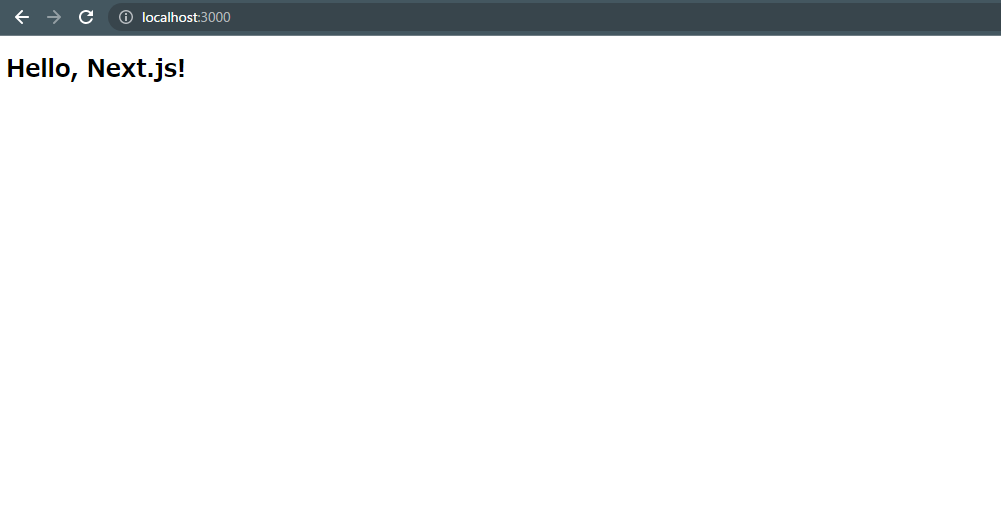
\includegraphics[width=12cm]{./image/03-Tech/chap4/01.png}
  \caption{Hello,Next.js}

\end{figure}




\subsection{LayoutとHead}

サーバを起動すると自動的にappディレクトリにlayout.tsx、head.tsxというファイルが作られていました。

next/headを使って各ページファイルにheadを定義していたのがhead.tsxに書けるようになったみたいですね。

\begin{tcblisting}{title={head.tsx},listing options={style=customstyle},listing only, breakable}
  export default function Head() {
      return (
      <>
        <title></title>
        <meta content="width=device-width, initial-scale=1" name="viewport" />
        <link rel="icon" href="/favicon.ico" />
      </>
      )
    }
\end{tcblisting}



ページの共通レイアウトを定義するファイル。




\begin{tcblisting}{listing options={style=customstyle},listing only, breakable}
  export default function RootLayout({
      children,
    }: {
      children: React.ReactNode
  }) {
      return (
        <html>
          <head />
          <body>{children}</body>
        </html>
      )
    }

\end{tcblisting}


今までは\_app.tsxなどに下記のようにレイアウトを定義していました。
\begin{tcblisting}{title={\_app.tsx},listing options={style=customstyle},listing only, breakable}
  <Layout>
    <Component {...pageProps} />
  </Layout>
\end{tcblisting}




この方法だとページごとにレイアウトを変えられないです。
なのでページごとにレイアウトを変えたい場合はgetLayoutを用いる必要がありました。
Next.js 13ではレイアウトを変えたいページがあるディレクトリにlayout.tsxを置けばページごとにレイアウトを変えられるようになりました。


ここではダッシュボードページのレイアウトの場合を考えます。
appディレクトリの中でdashbordディレクトリを作成して以下のようにlayout.tsxを配置するだけです。



\begin{tcblisting}{title={
        app/dashboard/layout.tsx
      },listing options={style=customstyle},listing only, breakable}
  export default function DashboardLayout({
      children,
    }: {
  children: React.ReactNode;
  }) {
      return <subsection>{children}</subsection>;
    }

\end{tcblisting}




少し疑問に思ったのがdashboardディレクトリのpage.tsxではRootLayoutは呼ばれずDashboardLayoutのみが呼ばれるのかと思っていました。しかし、実際には入れ子構造で呼び出されるようです。

公式の画像がわかりやすいので貼っておきます。
\begin{figure}[H]
  \centering
  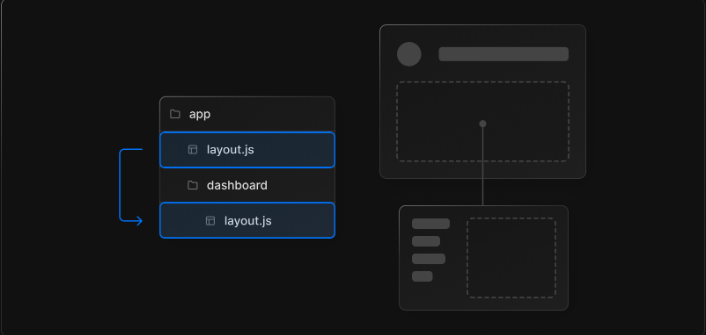
\includegraphics[width=12cm]{./image/03-Tech/chap4/02.png}
  \caption{layout.jsの適用範囲}
\end{figure}

次の機能に行く前にdashboardディレクトリにpage.tsxも作っておきます。
\begin{tcblisting}{title={
        app/dashboard/layout.tsx
      },listing options={style=customstyle},listing only, breakable}
  export default function DashBoardPage() {
      return <h1>DashBoard Page</h1>;
  }

\end{tcblisting}


違いがわかりやすいように他のファイルも変更します。
\begin{tcblisting}{title={
        app/layout.tsx
      },listing options={style=customstyle},listing only, breakable}
      export default function RootLayout({
        children,
      }: {
        children: React.ReactNode;
      }) {
        return (
          <html>
            <head />
            <body
              style={{
                backgroundColor: '#C0C0C0',
                padding: '50px',
              }}
            >
              {children}
            </body>
          </html>
        );
      }
      

\end{tcblisting}




\begin{tcblisting}{title={
        app/dashboard/layout.tsx
      },listing options={style=customstyle},listing only, breakable}
      export default function DashboardLayout({
        children,
      }: {
        children: React.ReactNode;
      }) {
        return (
          <subsection
            style={{
              backgroundColor: 'white',            
            }}
          >
            {children}
          </subsection>
        );
      }
\end{tcblisting}



ページの見た目が画像のようになってればOK。


\begin{figure}[H]
  \centering
  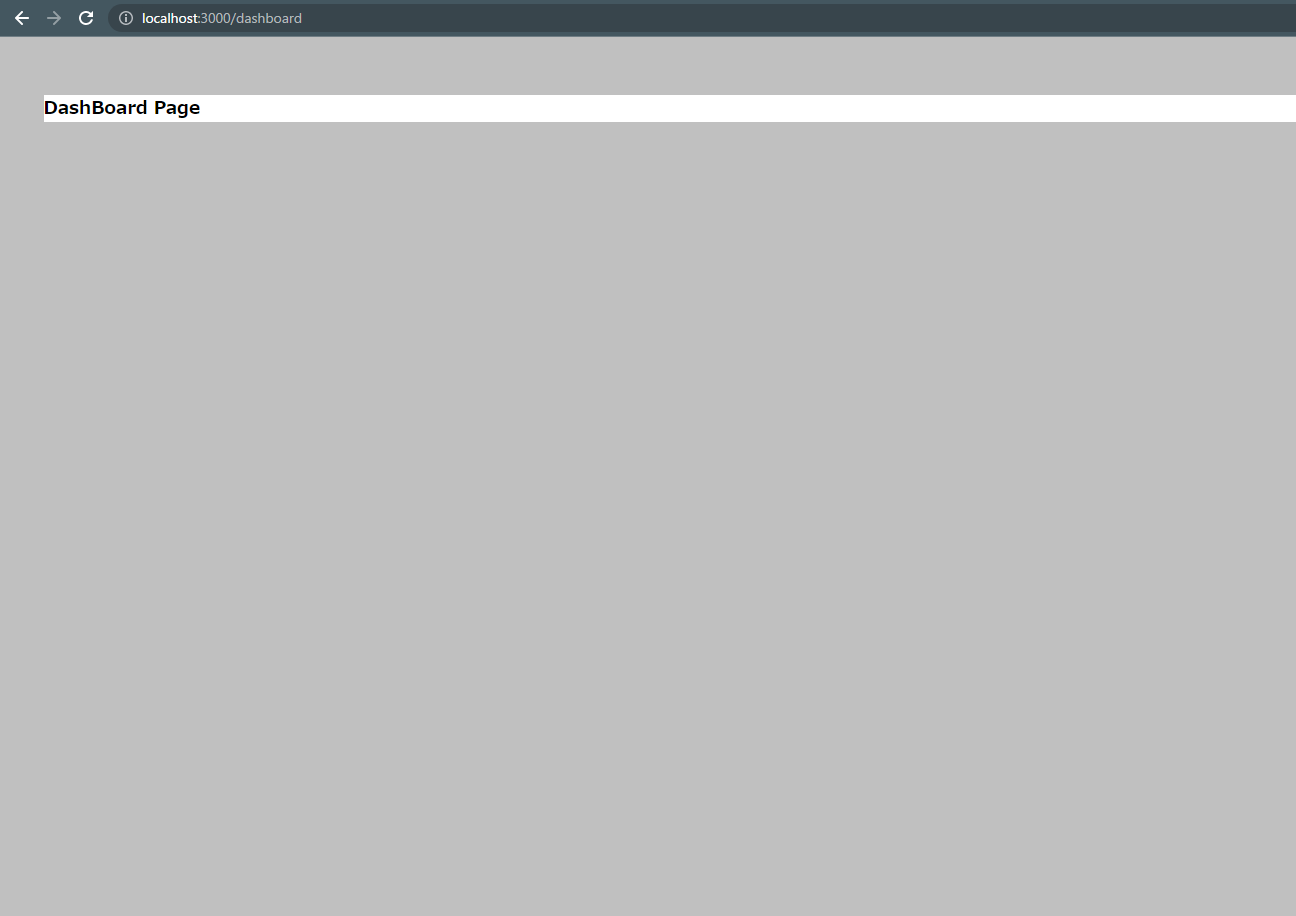
\includegraphics[width=12cm]{./image/03-Tech/chap4/03.png}
  \caption{DashBoardページ}
\end{figure}










\subsection{React Server Components}
React Server Components(RSC)はReact18で追加された機能でクライアントと
サーバ側が協調してアプリケーションをレンダリングできる機能です。
これによりコンポーネントごとに最適なレンダリング方法を選択できるようになります。
例えばデータの取得はサーバ側で行い,ユーザの操作によって変わる部分はクライアント側で
レンダリングできます。これも公式ドキュメントの図がわかりやすいので貼っておきます。


\begin{figure}[H]
  \centering
  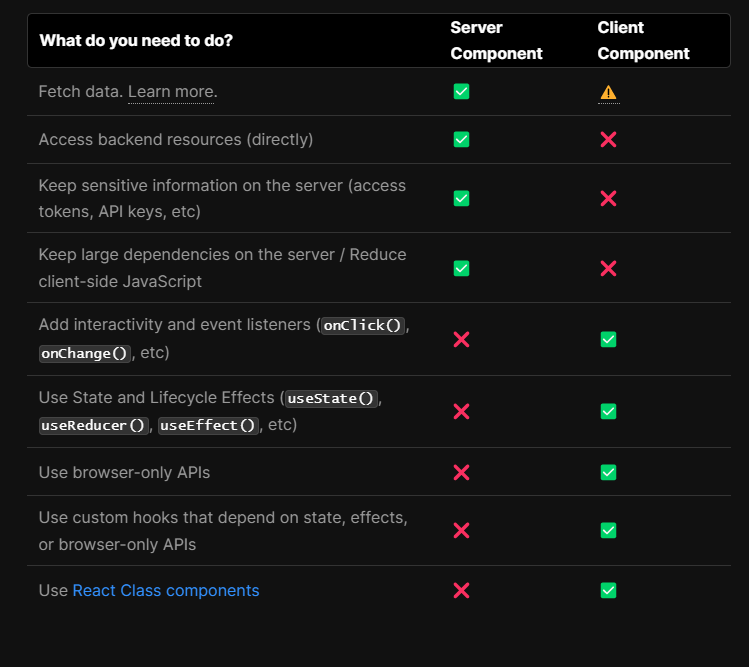
\includegraphics[width=12cm]{./image/03-Tech/chap4/04.png}
  \caption{Sever ComponentとClient Componentsの違い}
\end{figure}



またSSRとの違いとしてクライアント側のJavaScriptの量を減らせる点です。
SSRの場合ハイドレーション(サーバ側で生成したDOMとクライアントで生成したDOMを合成する)というステップがありページを早く表示できてもクライアント側でも同じ処理が走るためJavaScriptの量は同じでした。
RSCはサーバ側でレンダリングした後、残りをクライアント側でレンダリングします。これによってクライアント側に送信されるJavaScriptの量を減らせます。


\subsection{サーバーコンポーネントでデータを取得}


appディレクトリ内のコンポーネントはデフォルトだとサーバコンポーネントになっています。
以下のコードはサーバサイドでQiitaの記事リストを取得して表示するものです。
dashboard/page.tsxを書き換えます。



\begin{tcblisting}{title={
        dashboard/page.tsx
      },listing options={style=customstyle},listing only, breakable}
  type Article = {
    id: number;
    title: string;
  };

  async function getArticle(): Promise<Article[]> {
    const res = await fetch('https://qiita.com/api/v2/items?page=1&per_page=24');

    if (!res.ok) {
        throw new Error('Failed to fetch data');
    }

    return res.json();
  }

  export default async function DashBoardPage() {
    const articles = await getArticle();

    return (
      <div>
        <h1>Dashboard</h1>
        <div
        style={{
            display: 'flex',
            flexDirection: 'column',
            flexWrap: 'wrap',
            height: '50vh',
          }}
        >
          {articles?.map((article) => (
            <div
            key={article.id}
            style={{
                display: 'flex',
                gap: '10px',
              }}
            >
              <p>{article.title}</p>
            </div>
            ))}
        </div>
      </div>
    );
  }


\end{tcblisting}






画像のように表示される。

\begin{figure}[H]
  \centering
  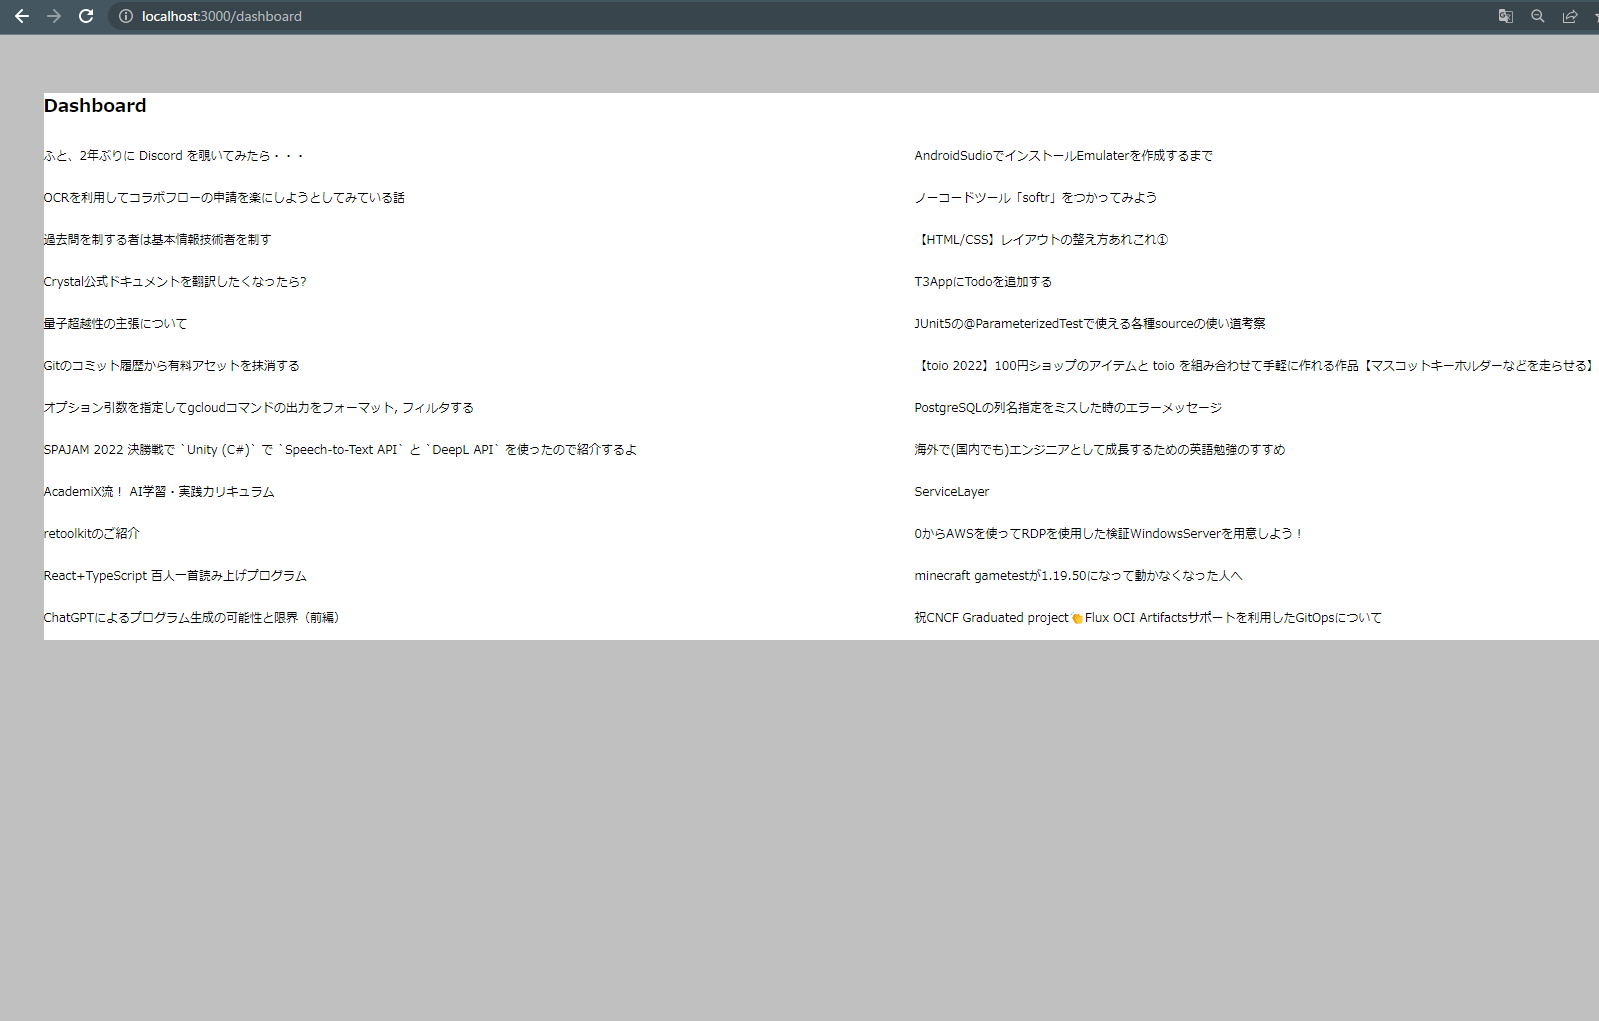
\includegraphics[width=12cm]{./image/03-Tech/chap4/06.png}
  \caption{APIからデータ取得後のページ}
\end{figure}


サイトにカーソルを合わせて右クリックしてページのソースを表示をクリックしてみましょう。
あらかじめデータが入った状態でサーバから送られてくるのでページソースに記事データが表示されています。

\begin{figure}[H]
  \centering
  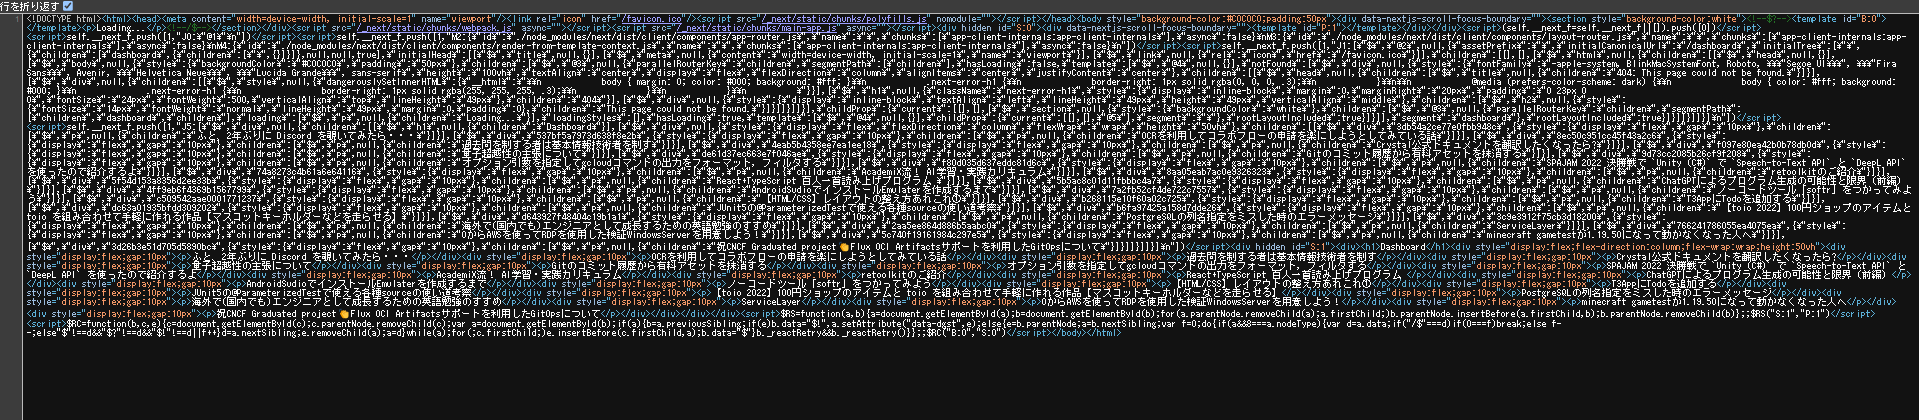
\includegraphics[width=12cm]{./image/03-Tech/chap4/05.png}
  \caption{ページのソース表示}
\end{figure}

\subsection{ローディングUI表示}

次はローディングUIを表示する機能です。
dashboradディレクトリにloading.tsxを作成します。

\begin{tcblisting}{title={
        loading.tsx
      },listing options={style=customstyle},listing only, breakable}
  export default function Loading() {
    return <p>Loading...</p>;
  }
\end{tcblisting}


データの取得が終わり、pageコンポーネントがレンダリングされるまでの間はLoadingコンポーネントが表示されます。

\begin{figure}[H]
  \centering
  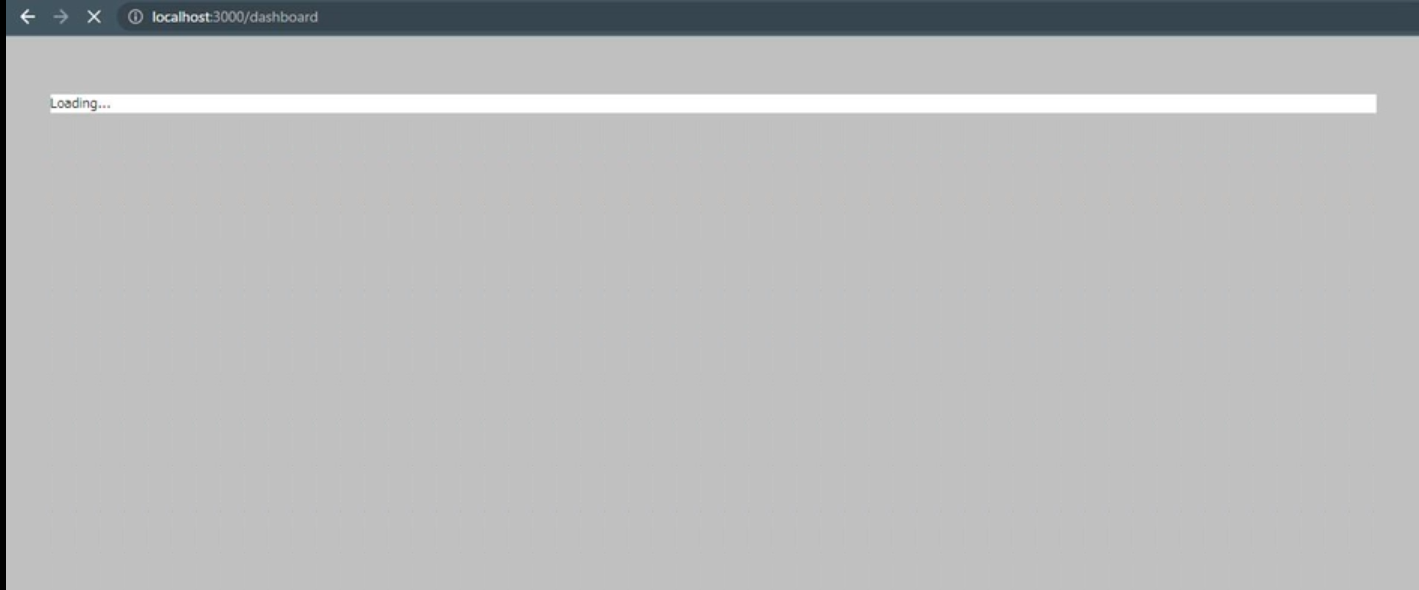
\includegraphics[width=12cm]{./image/03-Tech/chap4/07.png}
  \caption{ローディングUI}
\end{figure}




これはReact18で追加されたSuspenseという機能が使われていてます。
Suspenseについて説明するとコンポーネントが表示されるまでの状態を指定できるコンポーネントです。
非同期的なコンポーネントの場合レンダリングに時間がかかるためその間に何を表示させるかをSuspenseを使うと指定できるようになります。

具体的な使用例を上げます。下のコードはデータフェッチライブラリ React Queryを使ったデータ取得と表示のサンプルです。






\begin{tcblisting}{listing options={style=customstyle}, listing only, breakable}
  import { QueryClient, QueryClientProvider, useQuery } from 'react-query';

  const queryClient = new QueryClient();

  export default function App() {
    return (
    <QueryClientProvider client={queryClient}>
    <Example />
    </QueryClientProvider>
    );
  }
  export function Loading() {
      return <p>Loading...</p>;
  }

  function Example() {
    const { isLoading, data } = useQuery('repoData', () =>
    fetch('https://api.github.com/repos/tannerlinsley/react-query').then(
    (res) => res.json()
    )
    );

    if (isLoading) return <Loading />;

    return (
      <div>
        <h1>{data.name}</h1>
        <p>{data.description}</p>
      </div>
    );
  }
\end{tcblisting}




Suspenseを使えば下のコードに置き換えられます。


\begin{tcblisting}{listing options={style=customstyle},listing only, breakable}
import { Suspense } from 'react';
import { QueryClient, QueryClientProvider, useQuery } from 'react-query';

const queryClient = new QueryClient();

export default function App() {
  return (
    <QueryClientProvider client={queryClient}>
      {/* suspenseコンポーネントででラップ */}
      <Suspense fallback={<Loading />}>
        <Example />
      </Suspense>
    </QueryClientProvider>
  );
}
export function Loading() {
  return <p>Loading...</p>;
}

function Example() {
  const { data } = useQuery('repoData', () =>
    fetch('https://api.github.com/repos/tannerlinsley/react-query').then(
      (res) => res.json()
    )
  );
  //ローディングプロパティによる表示分岐の削除

  return (
    <div>
      <h1>{data.name}</h1>
      <p>{data.description}</p>
    </div>
  );
}

\end{tcblisting}





変更点はExampleコンポーネントをSuspenseコンポーネントでラップしているのと、Exampleコンポーネントの中のisLoadingプロパティを使った表示切替の部分が消えているところです。
Suspenseのいいところはデータ取得をするコンポーネントの中で表示を切り替える処理を書く必要がない所です。
これによってより宣言的なコードになりました。またコンポーネントの責務の観点から見てもローディング完了時の表示だけでよくシンプルになっています。

Next.js 13ではloading.tsxを置いてあげるとNext.js側がそれを読み取りPageコンポーネントをSuspenseコンポーネントでラップしてくれるようです。
普通に書くと以下のようになります。



\begin{tcblisting}{listing only, breakable}
  <Layout>
    <Headr/>
    <SideNav/>
    <Suspense fallback={<Loading />}>
      <DashBoardPage />
    </Suspense>
  </Layout>
\end{tcblisting}

ディレクトリ内にloading.tsxを配置すると、自動的にこのコードを記述した動作が実現されます。



\subsection{エラーハンドリング}

次にエラーハンドリングを見ていきます。
dashboardディレクトリにerror.tsxを作成します。


\begin{tcblisting}{title={
        dashboard/error.tsx
      },listing options={style=customstyle},listing only, breakable}
'use client';

import { useEffect } from 'react';

export default function Error({
  error,
  reset,
}: {
  error: Error;
  reset: () => void;
  }) {
  useEffect(() => {
  // Log the error to an error reporting service
  console.error(error);
  }, [error]);

  return (
  <div>
    <p>Something went wrong!</p>
    <button onClick={() => reset()}>Reset error boundary</button>
  </div>
  );
}
\end{tcblisting}



公式ドキュメントによるとerror.tsxはクライアントコンポーネントである必要がありuse client;と書けばクライアントコンポーネントして利用するできるようです。
loading.tsxと同じようにファイルを置いておけば自動的にPageをネストしてエラーハンドリングをしているようです。

普通に書いた場合


\begin{tcblisting}{title={
  dashboard/error.tsx
},listing options={style=customstyle},listing only, breakable}
<Layout>
    <Headr/>
    <SideNav/>
    <ErrorBoundary fallback={<Loading />}>
      <DashBoardPage />
    </ErrorBoundary>
</Layout>
\end{tcblisting}



ただこれを見てわかる通りpageをラップしてるので同階層のコンポーネントのエラーハンドリングはできない感じですね.したいならより上の階層でErrorBoundaryを使う必要がありそうです。

実際にコードを書き換えてエラーを出してみます。
存在しないURL'hoge'を指定しgetArticleでしていたエラーハンドリングを削除しています。


\begin{tcblisting}{title={

        dashboard/page.tsx
      },listing options={style=customstyle},listing only, breakable}

'use client';

import { useEffect } from 'react';
      
export default function Error({
  error,
  reset,
}: {
  error: Error;
  reset: () => void;
}) {
  useEffect(() => {
    // Log the error to an error reporting service
    console.error(error);
  }, [error]);
      
  return (
    <div>
      <p>Something went wrong!</p>
      <button onClick={() => reset()}>Reset error boundary</button>
    </div>
  );
}

\end{tcblisting}


エラーの内容とエラーページが表示されていますね。


\begin{figure}[H]
  \centering
  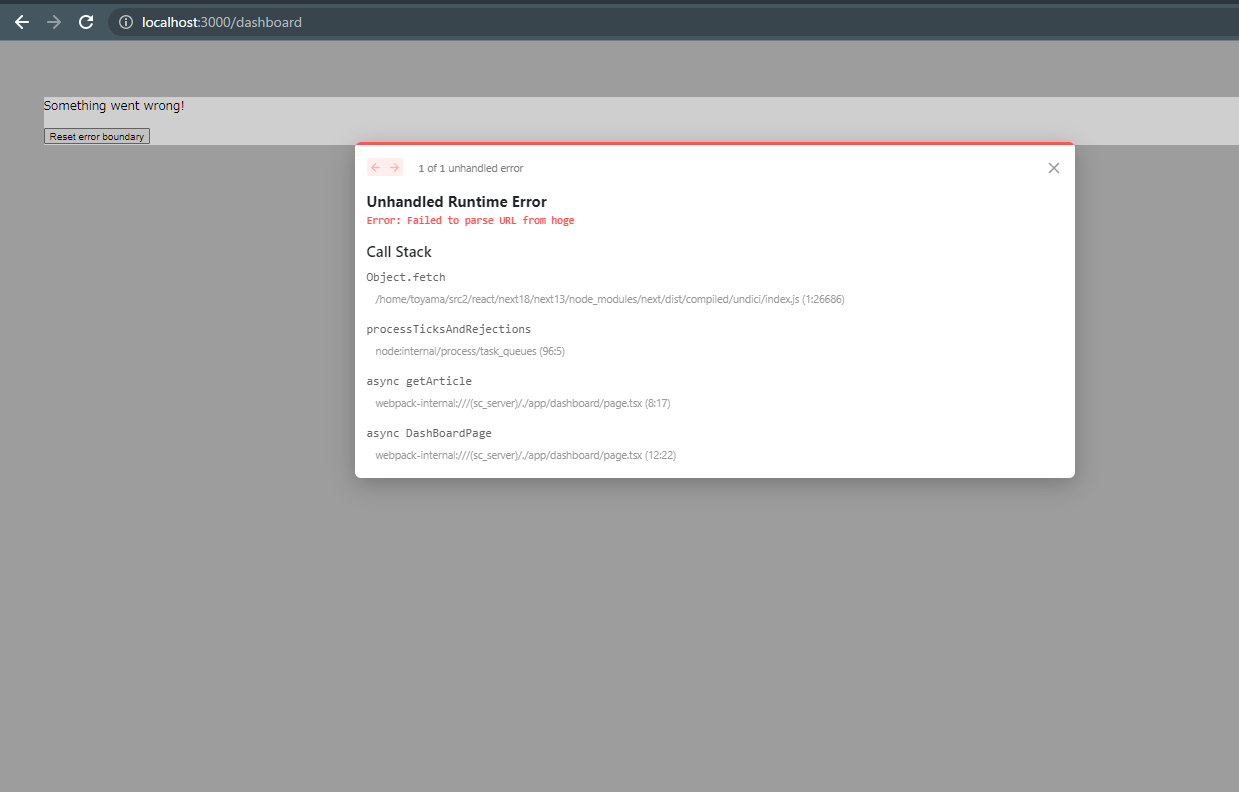
\includegraphics[width=12cm]{./image/03-Tech/chap4/08.png}
  \caption{エラーハンドリング画面}
\end{figure}



\subsection{終わりに}
感想としては、Next.js 13の機能はReact18のSupenseやRSCなどの機能に合わせたアップデートというのを強く感じました。